\section{The Large Hadron Collider}
The Large Hadron Collider (LHC)~\ref{cern-faq} is the largest and most powerful particle collider that has ever been built. Construction of the LHC involved a collaboration of more than 10,000 scientist from more than 100 countries and was completed in 2008, after a decade of work. The cost of the machine alone is about 5 billion USD (3 billion Euro).

The European Organization for Nuclear Research (CERN) built the LHC in a tunnel underneath the border of France and Switzerland, near the city of Geneva. The LHC occupies a large tunnel 27 km in circumference that was originally constrcted in the 1990s for the Large Electron Positron collider (LEP). Hadrons (either protons or ions) are accelerated and focused into two beams traveling in opposite directions around this tunnel. These beams are then made to collide with very high energy at one of the four collision points along the ring where their paths intersect. AEach of these points is home to one of the four main LHC experiments: A Large Ion Collider
Experiment (ALICE)~\cite{cern-jinst-alice}, ATLAS~\cite{cern-jinst-atlas}, the Compact Muon Solenoid (CMS)~\cite{cern-jinst-cms}, and the Large Hadron Collider beauty (LHCb) experiment~\cite{cern-jinst-lhcb}. ALICE is a detector that looks at collisions of lead ions to study the properties of quark-gluon plasma. ATLAS is a general-purpose detector that looks for a wide range of possible new types of physics, including the Higgs boson, supersymmetry (SUSY) and extra dimensions. CMS is an additional general-purpose detector, designed and run independently from ATLAS, but with the same goals in mind. LHCb is a detector specially designed to study the asymmetry between matter and anti-matter in the interactions of B-particles. Figure~\ref{fig:lhc-exp} shows a aerial view diagram with the locations of these four experiments along the LHC ring. The location of the LHC ring in relation to the city of Geneva and the French-Swiss border is also illustrated.

\begin{figure}[tp]
  \centering
  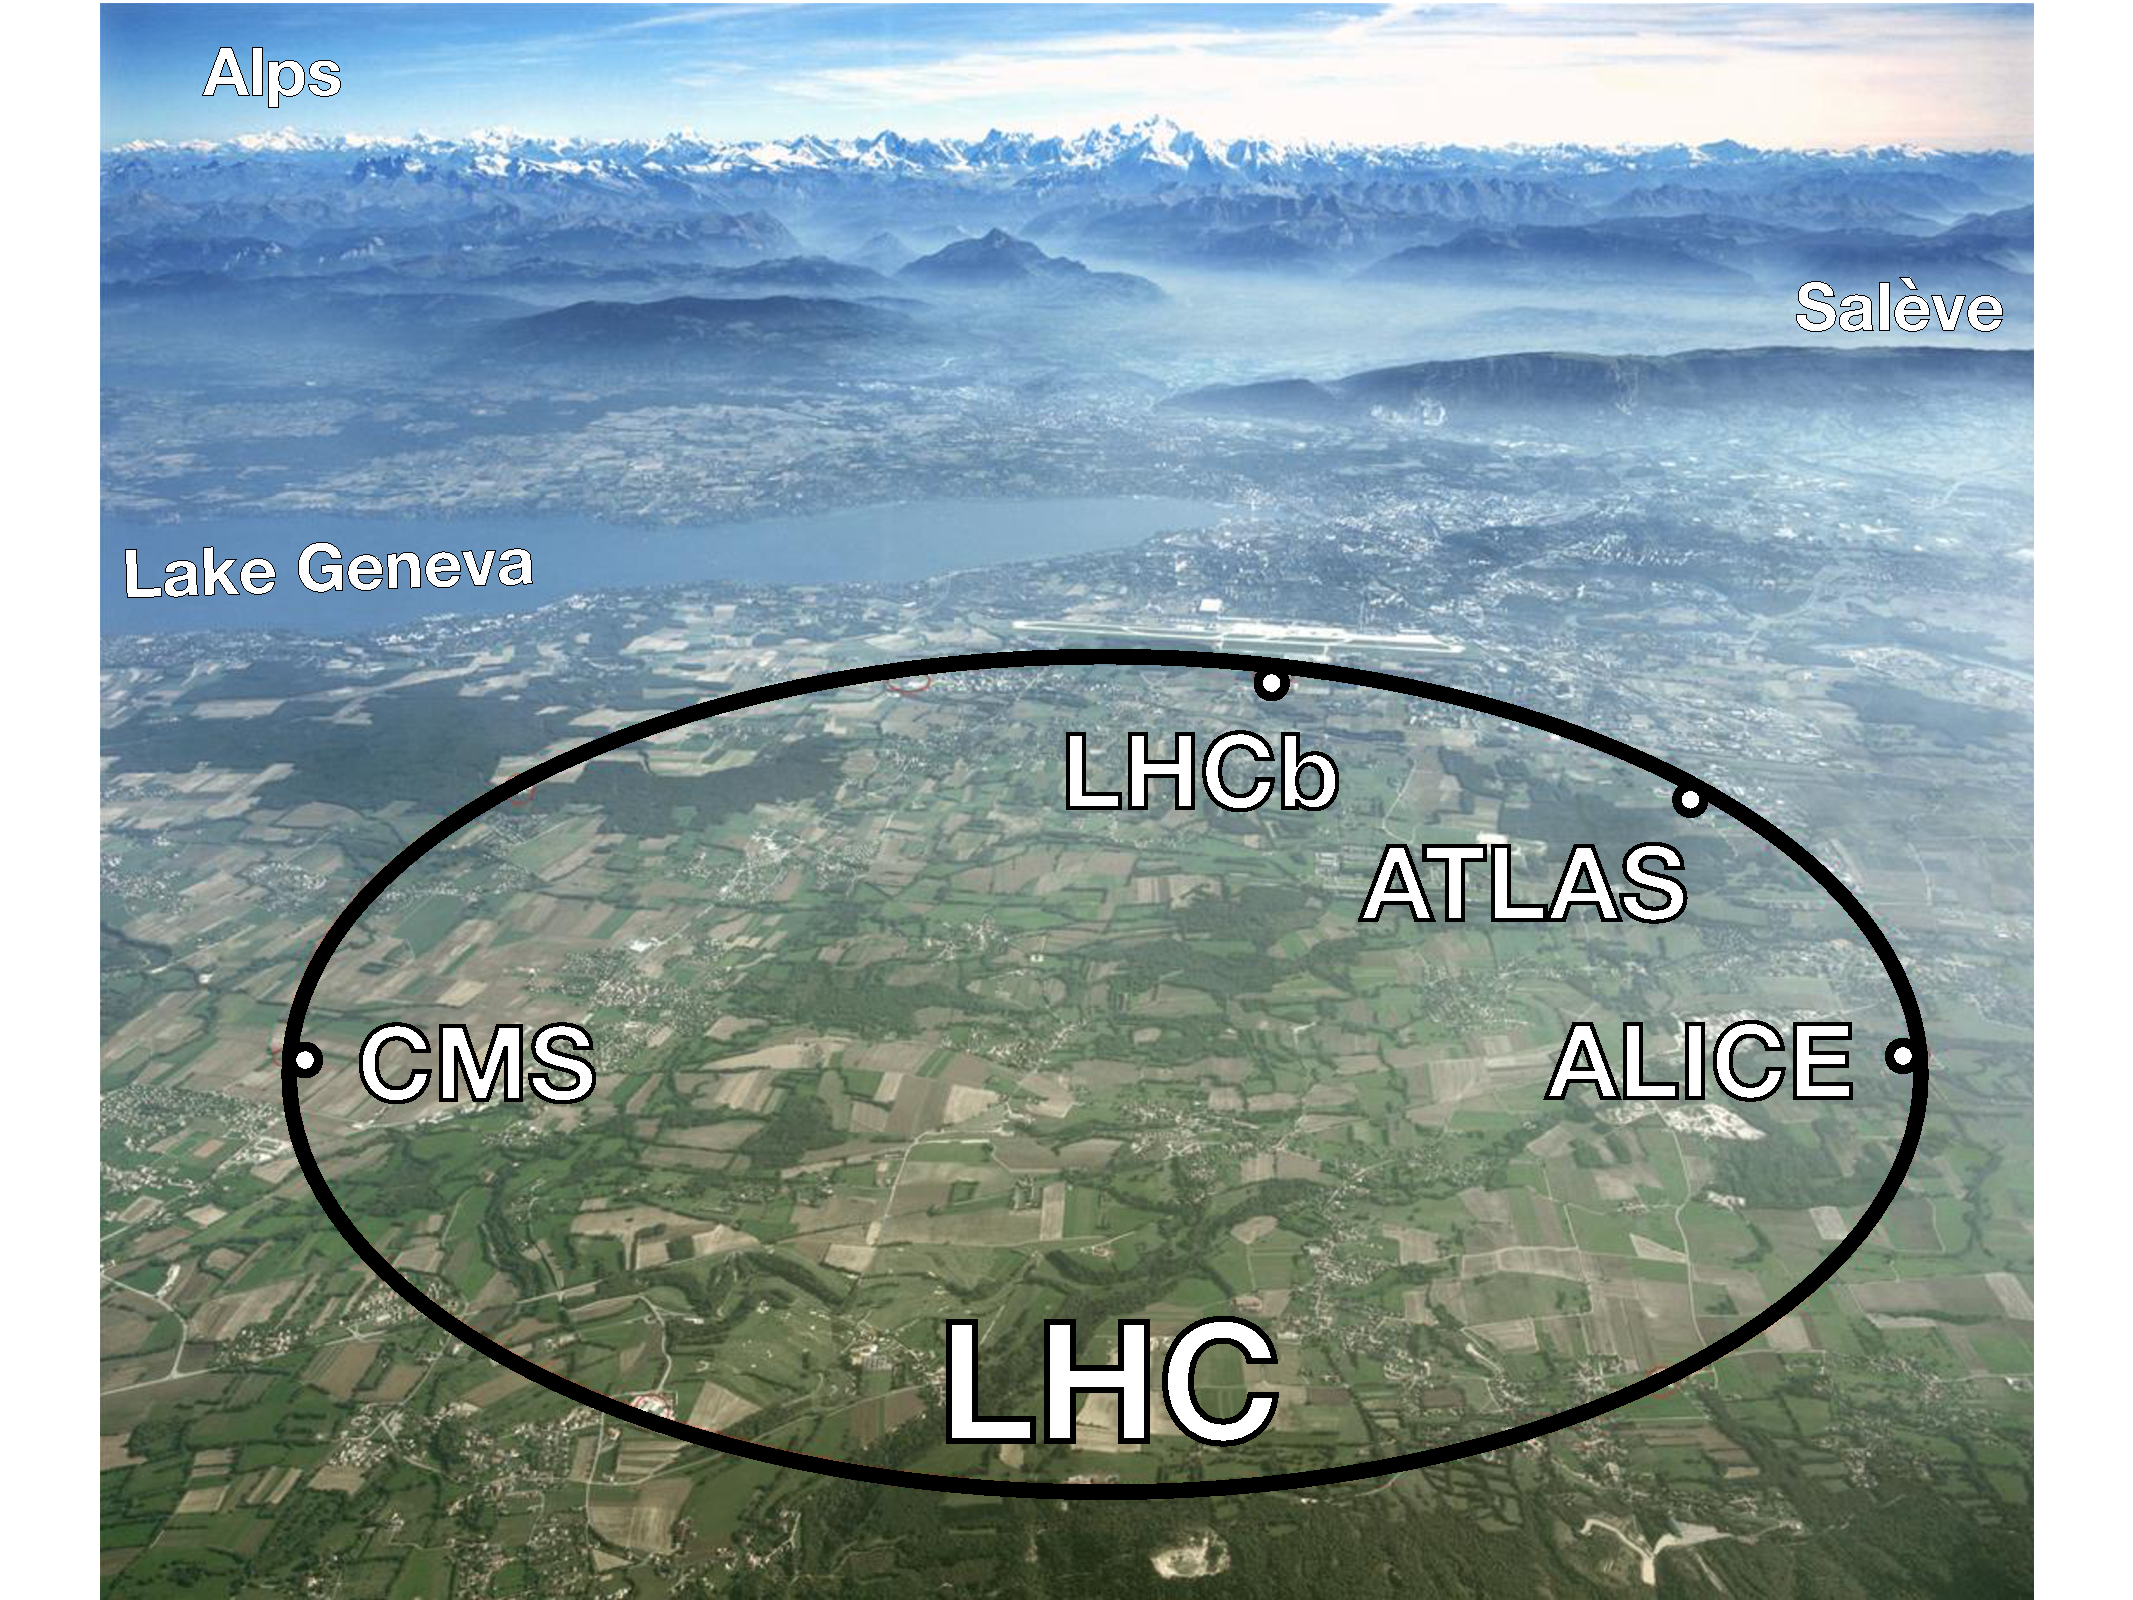
\includegraphics[width=0.90\textwidth]{fig/atlas/lhc-aerial.pdf}
  \caption{The location of the four main LHC experiments: ALICE, ATLAS, CMS and LHCb. The LHC tunnel is 27 km in circumference, situated underneath the border of France and Switzerland, near the city of Geneva, as shown.~\cite{atlas-surface}.}
  \label{fig:lhc-exp}
\end{figure}

The main goal of the LHC is to investigate unsolved questions in our current understanding of particle physics, such as the details of the Higgs mechanism, the existence of new particles from SUSY or extra dimensions and the source of dark matter and dark energy.
\subsection{Accelerator Complex}
A succession of machines known as the \emph{accelerator complex} accelerate particles to increasingly higher energies~\cite{cern-jinst-lhc}, shown in Figure~\ref{fig:lhc-chain}. First, an electric field is used to strip protons from atoms in a simple bottle of hydrogen gas. Then, the first accelerator in the chain, Linac 2, accelerates protons to 50 \mev. Next, the beam is injected into the Proton Synchrotron Booster (PSB) and then the Proton Synchrotron (PS), which accelerate the protons to 1.4 \gev and 25 \gev respectively. After that, the Super Proton Synchrotron accelerates the protons to 450 \gev. The last step in the chain is the LHC; from the SPS, protons are transferred into the two beam pipes of the LHC and accelerated in opposite direction. Filling each of the rings of the LHC takes 4 minutes and 20 seconds, and it takes another 20 minutes to accelerate each beam to its final energy of 4 \tev. The same two beams will circle for many hours.

Inside the LHC, the beams travel in opposite directions around separate rings called \emph{beam pipes} (or beamline), which are tubes kept at ultrahigh vacuum. The beams are directed by a collection of very strong superconducting electromagnets, including 1232 dipole magnets and 392 quadrupole magnets. Superconduction requires the magnets to be cooled to -271.3 C. A distribution system of liquid helium keeps the magnets cool. The 15 meter long dipole magnets steer the beams around the ring, while the 5-7 meter long quadrupole magnets focus the beams before collision. The protons in the beams circulate in well-defined groups called \textit{bunches}. Each bunch consists of approximately $10^{11}$ particles, and each beam has 2808 bunches. This bunch structure maximizes the chances of collisions since multiple protons have the chance to collide each crossing. In 2012, bunch crossings occurred every 50 nanoseconds.




\begin{figure}[tp]
  \centering
  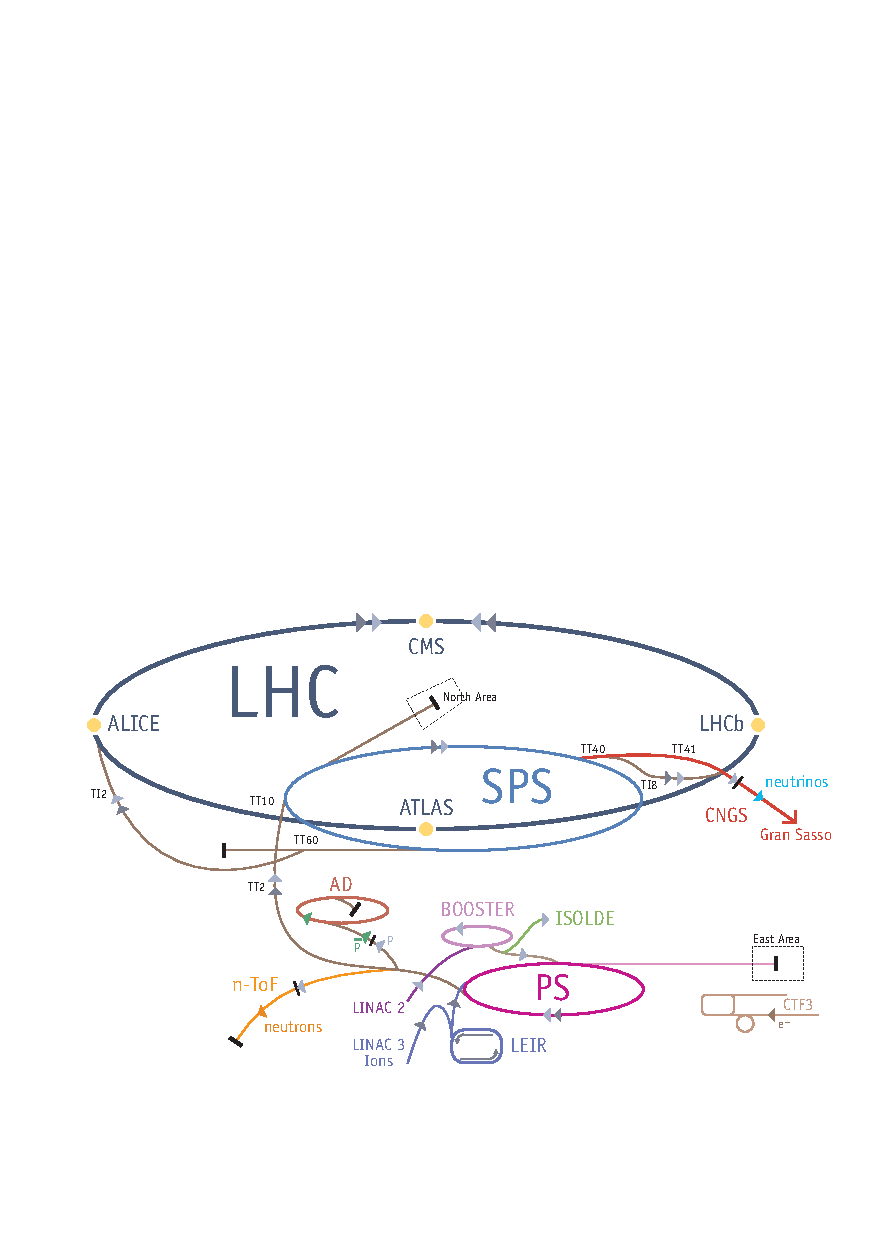
\includegraphics[width=0.90\textwidth]{fig/atlas/accel-chain.pdf}
  \caption{The LHC accelerator complex boosts particles to increasingly higher energies before reaching the LHC. The particle beams are accelerated successively by Linac 2, the Proton Synchrotron Booster (PSB), the Proton Synchrotron (PS), the Super Proton Synchrotron (SPS) and then finally enter the LHC rings~\cite{cern-faq}.}
  \label{fig:lhc-chain}
\end{figure}
\section{Beam conditions}
Due to the Radio Frequency (RF) fields in the accelerating cavities, the proton beams are segmented into groups of protons called \textit{bunches}. Each beam contains 2808 bunches, and each bunch contains 1.7$\times$10$^{11}$ protons. Many protons are included per bunch to maximize the probability of a proton-proton collision for a given bunch crossing. A bunch crossing occurred every 50 nanoseconds during operations in 2012.

Given two equally bunched beams, the instantaneous \textit{luminosity} ($\mathcal{L}$) is given by:
\begin{equation}\label{eqn:lumi}
  \mathcal{L} = f \frac{n_1 n_2}{4\pi \sigma_x\sigma_y},
\end{equation}
where $f=\SI{11245.5}{\hertz}$ is the collision frequency of the LHC beams; $n_{1}$ and $n_{2}$ are the numbers of protons in each beam; and $\sigma_{x}$ and $\sigma_{y}$ are the RMS beam widths in the horizontall (bend) and vertical directions.\cite{PDG} The maximum instantaneous luminosity of the LHC in 2012 was 7.7$\times$10$^{33}$

The instaneous luminosity must be integrated over time because the beam conditions that go into Equation~\ref{eqn:lumi} are always changing over the duration of a run. The integral over time and varied beam conditions is called the integrated luminosity and can be used to relate the number of events $N$ for a given physics process to its cross section $\sigma$:
\begin{equation}\label{eqn:nevt}
  N = \sigma \times \int{\mathcal{L}(t) dt}
\end{equation}
In 2012, the total integrated luminosity of the LHC was 20.3$^{-1}$fb with uncertainty of 2.8\% \cite{Lumi}. The cumulative luminosity recorded over the course of 2012 is shown in Figure~\ref{fig:2012lumi}.
\begin{figure}[tp]
  \centering
  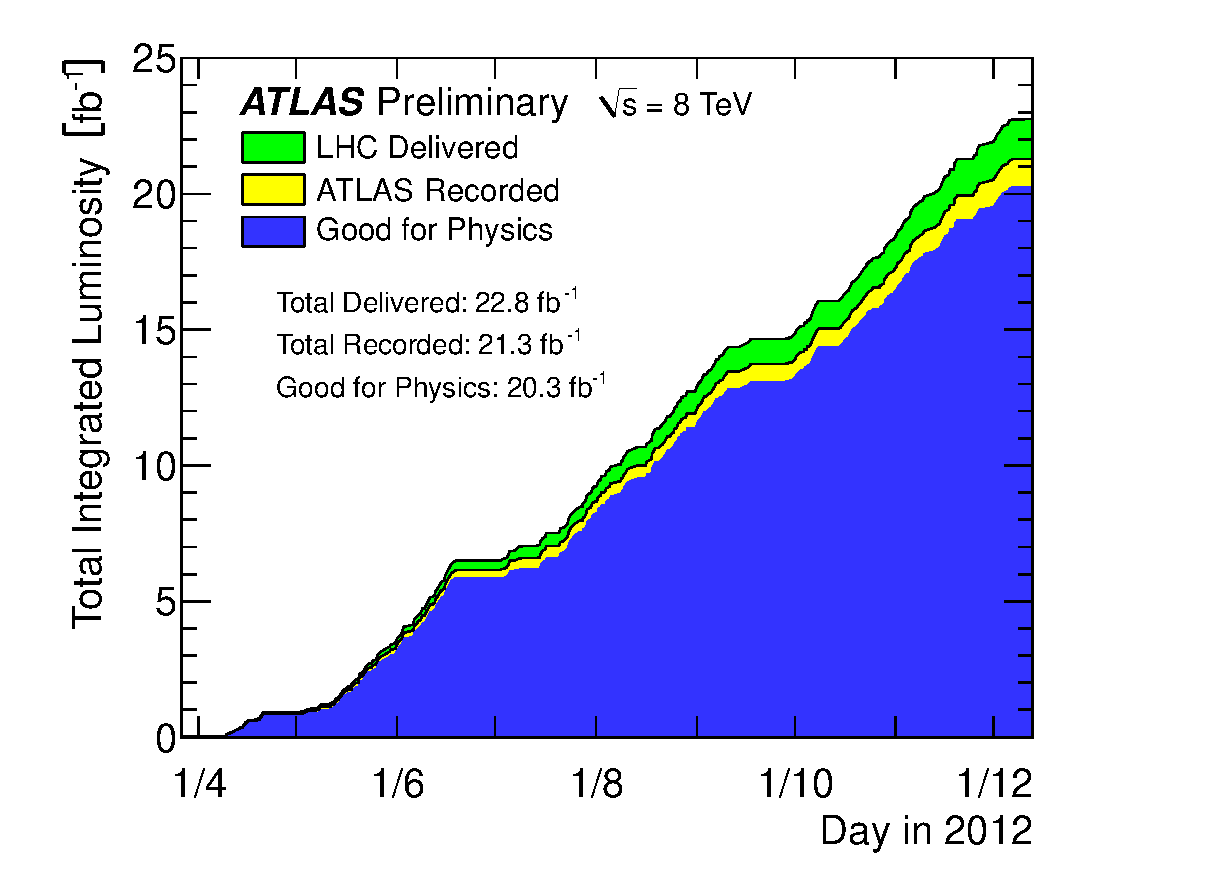
\includegraphics[width=0.90\textwidth]{fig/atlas/intlumivstime2012DQ.eps}
  \caption{Cumulative luminosity versus time delivered to (green), recorded by ATLAS (yellow), and certified to be good quality data (blue) during stable beams and for pp collisions at 8 TeV centre-of-mass energy in 2012. Luminosity can be lost due to data acquisition inefficiency or other effects.}
  \label{fig:2012lumi}
\end{figure}

The beam conditions also determine the number of proton-proton interactions that occur in each bunch crossing. When a single bunch crossing produces multiple separate proton-proton collisions, these events are referred to as \textit{pile-up}. Pile-up presents a signifigant challenge since it can rapidly increase the combinatoric complexity of reconstructing events and quickly degrades the performance of the reconstruction algorithms. In 2012, pile-up was much larger than anticipated. Figure~\ref{fig:pileup} shows the mean number of interactions per bunch crossing for 2011 and 2012, demonstrating the substantial increase of pile-up events in the latter. Reconstruction challenges were overcome by optimizing the existing reconstruction algorithms, as well as new techniques for subtracting pile-up events from the physics of interest. Pile-up techniques used in this analysis will be discussed in the chapter on object selection.

\begin{figure}[tp]
  \centering
  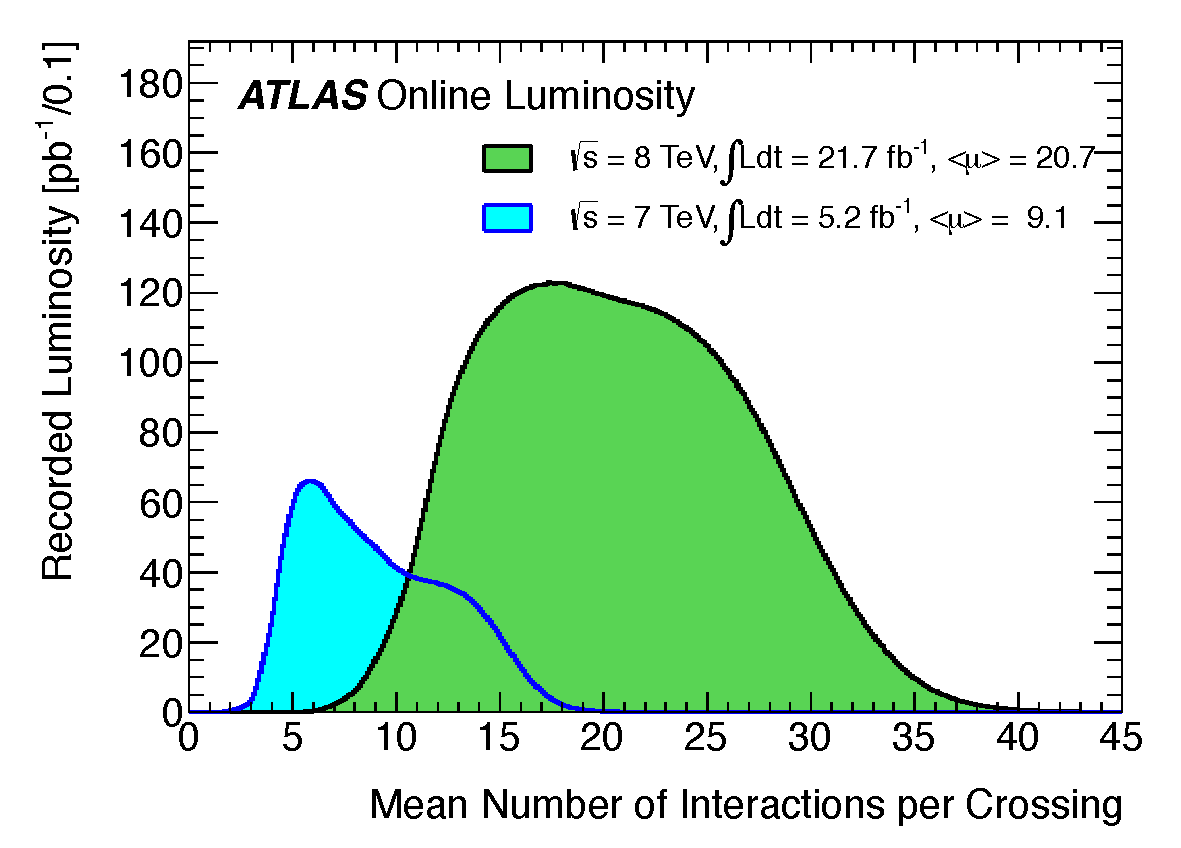
\includegraphics[width=0.90\textwidth]{fig/atlas/pileup.pdf}
  \caption{Luminosity-weight distribution of the mean number of interactions per bunch crossing. Both the full data from the 2011 and 2012 $pp$ runs at the LHC are shown.}
  \label{fig:pileup}
\end{figure}



\section{Overview of the ATLAS detector}
The ATLAS detector is a general purpose detector centered over one of the four interaction points of the LHC. The detector is cylindrical in shape with a diameter of 25 meters, a length of 46 meters and a weight of 7,000 tons; it contains around 100 million electronic channels and around 3,000 km of cables. Assembling the detector at CERN took 5 years and was completed in 2008. A schematic rendering of the ATLAS detector is shown in Figure~\ref{fig:atlas-cgi}.

In order to detect a wide range of physics in proton-proton collisons, ATLAS must measure the trajectory and energy of many different kinds of particles, including electron, muons, photons, kaons, protons and neutrons. Once these stable final-state particles are identified, information about the heavier, unstable particles can be inferred. This process is called \emph{reconstruction} and is discussed in detail in Chapter~\ref{ch:objects}.

ATLAS consists of specialized subdetectors designed to capture different phenomena. These subdetectors are arranged as increasingly larger cocentric cylinders around the interaction point (IP) where the LHC proton beams collide. There are three main specialized sub-systems: the \emph{inner detector} (ID),
, which is located just outside the beamline and uses silicon and transition radiation systems to track the trajectory of charged particles; the \emph{calorimeters}, which is located radially outward from the ID and designed to measure the energy of particles with a shower sampling method; and the \emph{muon system}, which is located farthest from the IP and measures muon momentum. Details of the subdetectors will be explored below. An overview of interaction of different types of particles with the subdetectors as they travel through the detector is illustrated in Figure~\ref{fig:atlas-wedge}.

In addition to the subdetector, ATLAS has a magnet system that bends the trajectory of charged particles as  they travel through the ATLAS detector. This allows the particle's momentum to be precisely calculated using the classical Lorentz force equation. The magnet system consists of a double configuration. Just outside the ID is a solenoidal magnet that produces a field of approximately 2 Tesla. A large toroidal magnet within the outermost part of the detector produces a 1-2 Tesla field.


\subsection{Coordinate system}


ATLAS uses a right-handed coordinate system with its origin at the IP in the center of the detector, which is illustrated in Figure~\ref{fig:atlas-coord}. The $z$-axis along the beamline with the positive direction counter-clockwise around the LHC. The $x-y$ plane is defined such that the coordinate system is right-handed, with the $x$-axis pointing from the IP to the center of the LHC, and the $y$-axis pointing upwards. This plane is usually referred to as the transverse plane, since it is perpendicular to the beamline. Cylindrical coordinates, $r$ and $\phi$, are used in the transverse plane with $\phi$ defined as the azimuthal angle around the beamline. Instead of the polar angle from the beamline, $\theta$, pseudorapidity is typically used and can be defined as:
\begin{equation}
\eta = -\text{ln}(\text{tan}\frac{\theta}{2})
\label{eq:eta}
\end{equation}
The pseudorapidity is used because in the limit of a massless particle, it is invariant with respect to Lorentz boosts along the beamline. Then, solid angle distances $\Delta R$ can be measured with the difference in pseudorapidity and azimuthal angle:
\begin{equation}
\Delta R = \sqrt{\Delta \phi^2 + \Delta \eta^2}
\label{eq:dR}
\end{equation}

% \subsection{Magnets}


%  The solenoid magnet is placed inside the electromagnetic (EM) calorimeter. This is different from most other detector designs where the magnet is placed outside the EM calorimeter. The advantage of the small solenoid is a compact design. A small magnetic field in the EM calorimeter also reduces the transverse spread of showers. The major problem is the increased amount of material in front of the calorimeter which causes many particles to start showering before they reach the active part of the calorimeter.
% The solenoid is a superconducting magnet kept at 4.5 K. To reduce the material the magnet does not have a separate cryostat but rather it shares the cryostat with the liquid argon calorimeter thus saving two cryostat walls. The half length of 2.65 m is considerably shorter than the inner tracking detector. This is a result of a compromise: a short coil reduces the material in front of the calorimeter; a long coil makes the magnetic field more uniform in the Inner Detector. The magnetic field along the z-direction drops from 2 T at the interaction point to around 0.5 T at the end of the Inner Detector.

% The toroid magnet system is divided into one barrel part and two forward systems. With a toroid field, particles will across the complete pseudorapidity range, be almost perpendicular to the field. This means that the field integral  $\int$Bdl , which is the important factor for momentum resolution, can be kept high even in the forward direction. The structure is open with 8 coils in the central region each in separate cryostats. One of the rectangular shaped cryostats can be seen in the front of fig. 4.1. In the forward direction the toroid field is also formed by 8 superconducting coils but there placed in a common cryostat.

% The low number of coils to form the toroid field results in a field strength that varies strongly with the  $\phi$ coordinate. The field integral varies in the barrel from 2-6 Tm and in the end-caps from 4-8 Tm. This is not ideal but an economical necessity.

\begin{figure}[tp]
  \centering
  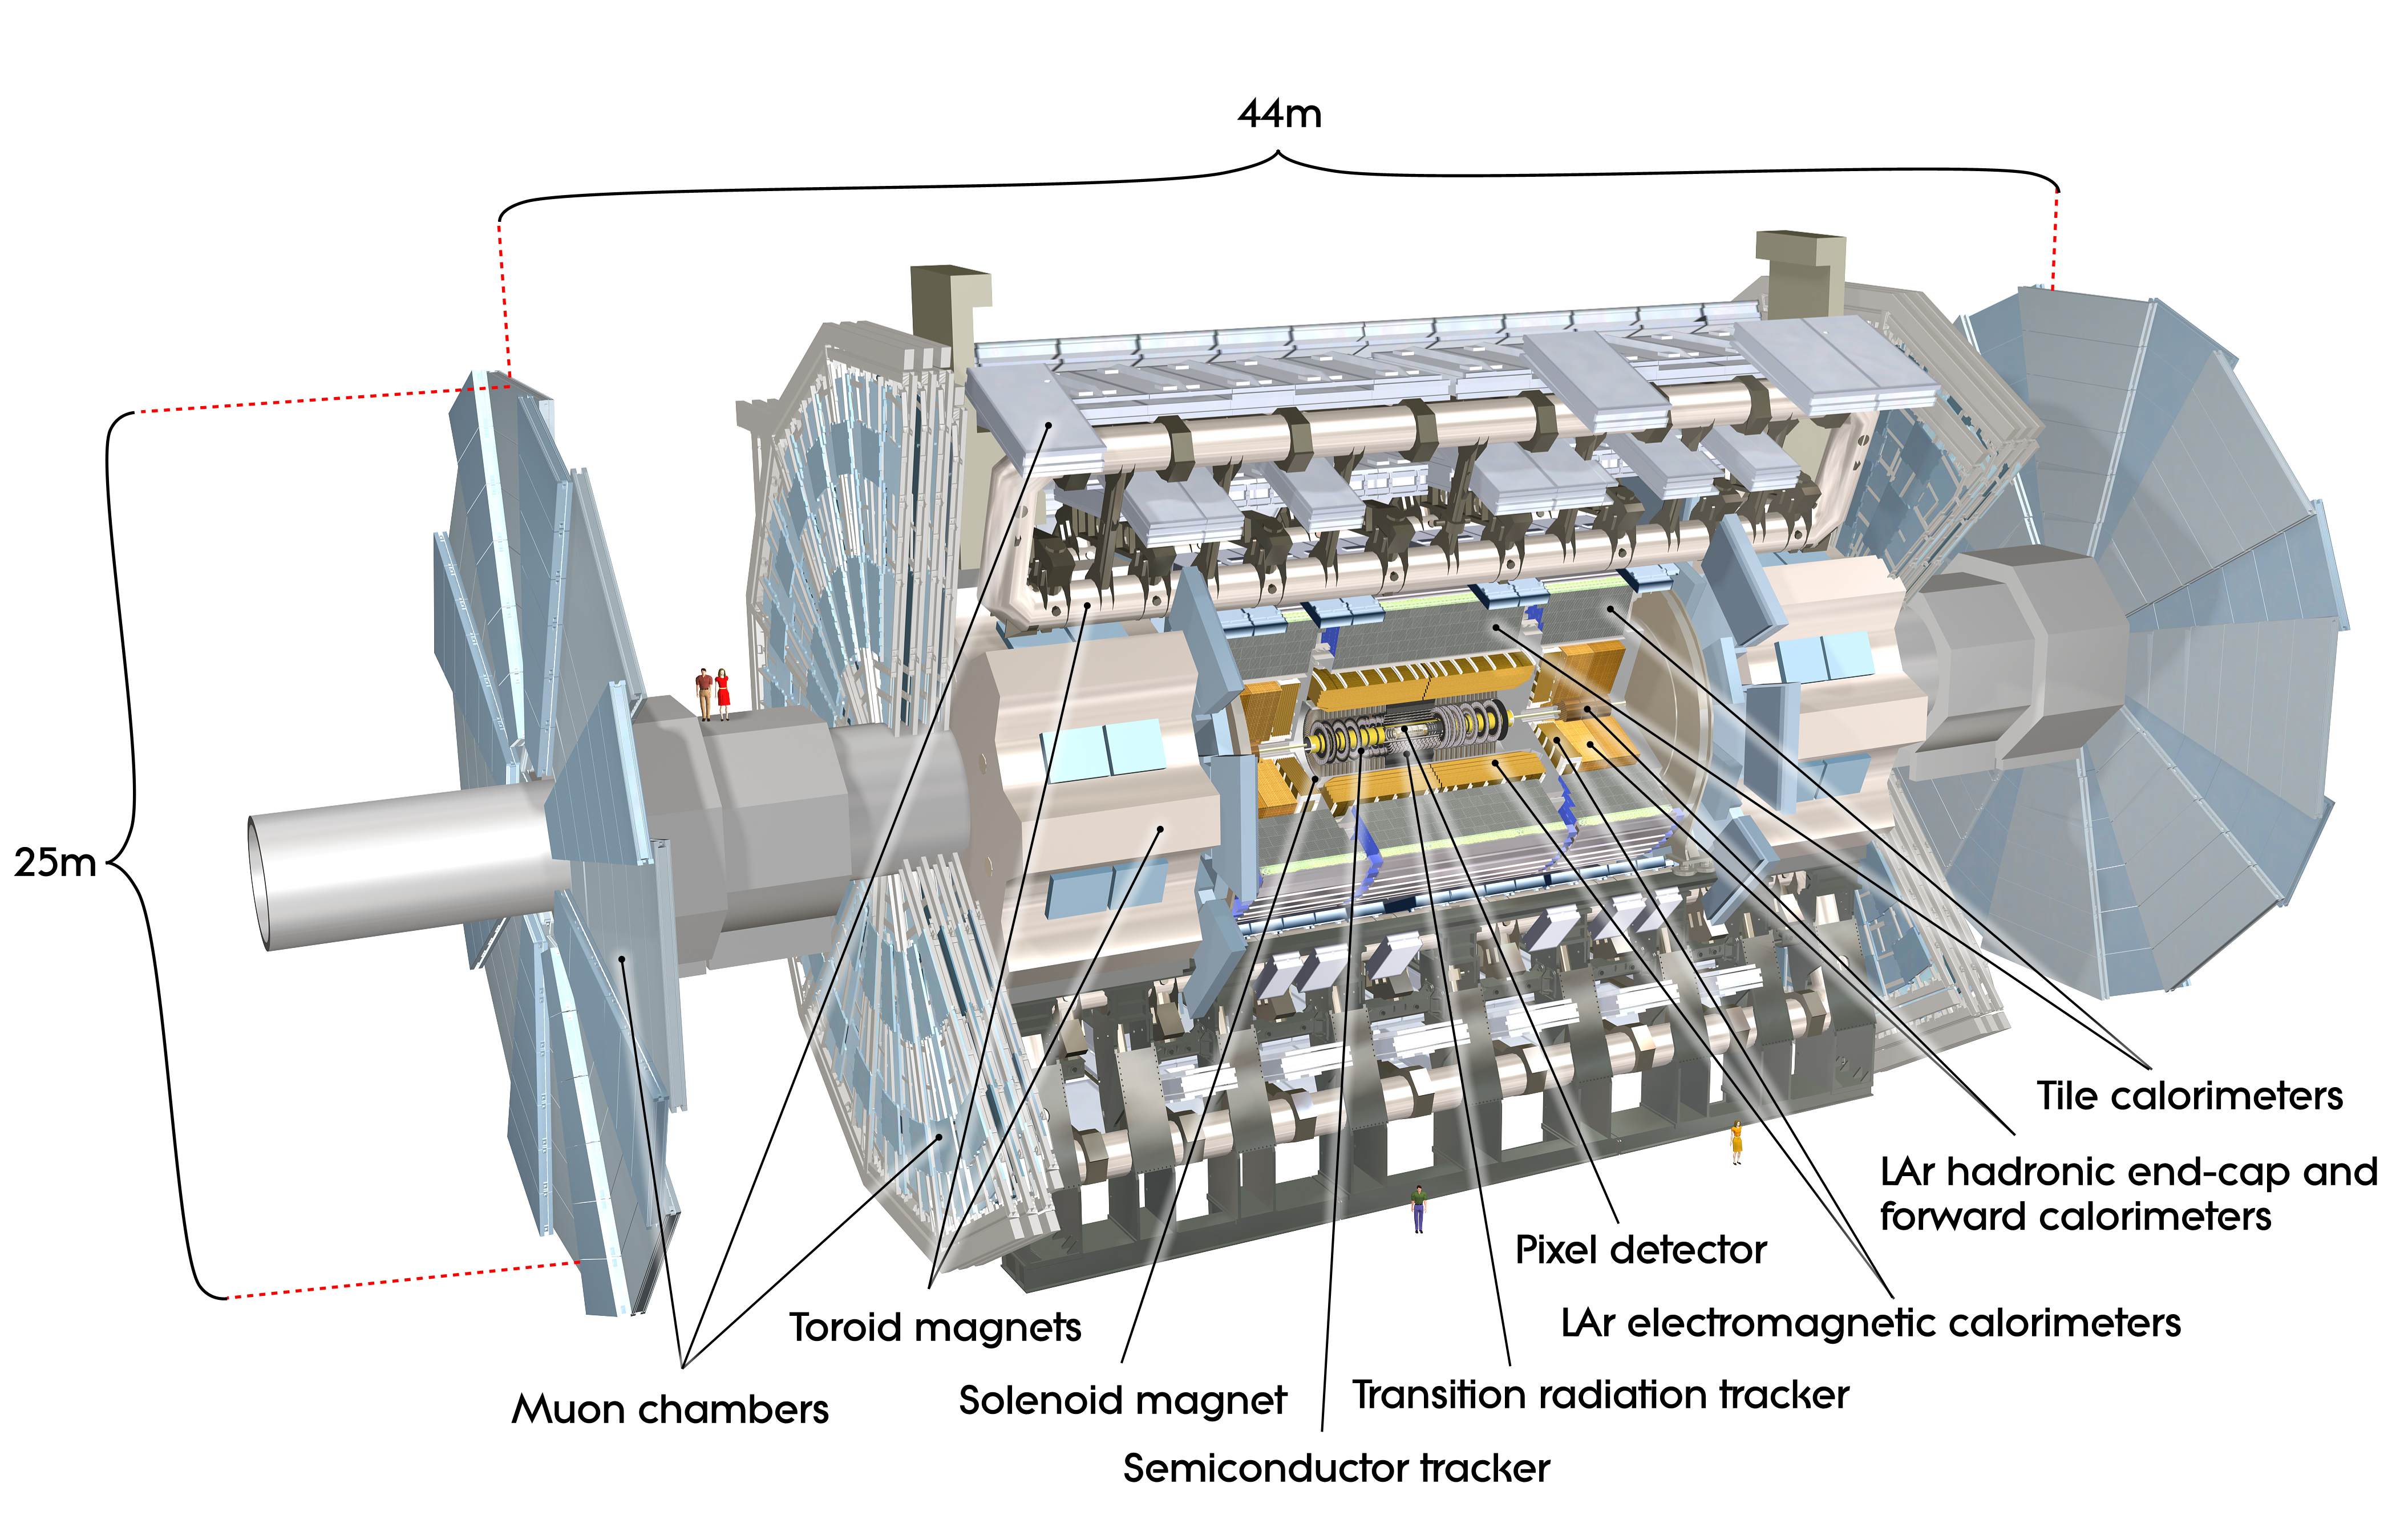
\includegraphics[width=0.90\textwidth]{fig/atlas/atlaspic.jpg}
  \caption{Computer generated illustration of the whole ATLAS detector detector, with various subdetectors highlighted\cite{Pequenao:1095924}.}
  \label{fig:atlas-cgi}
\end{figure}

\begin{figure}[tp]
  \centering
  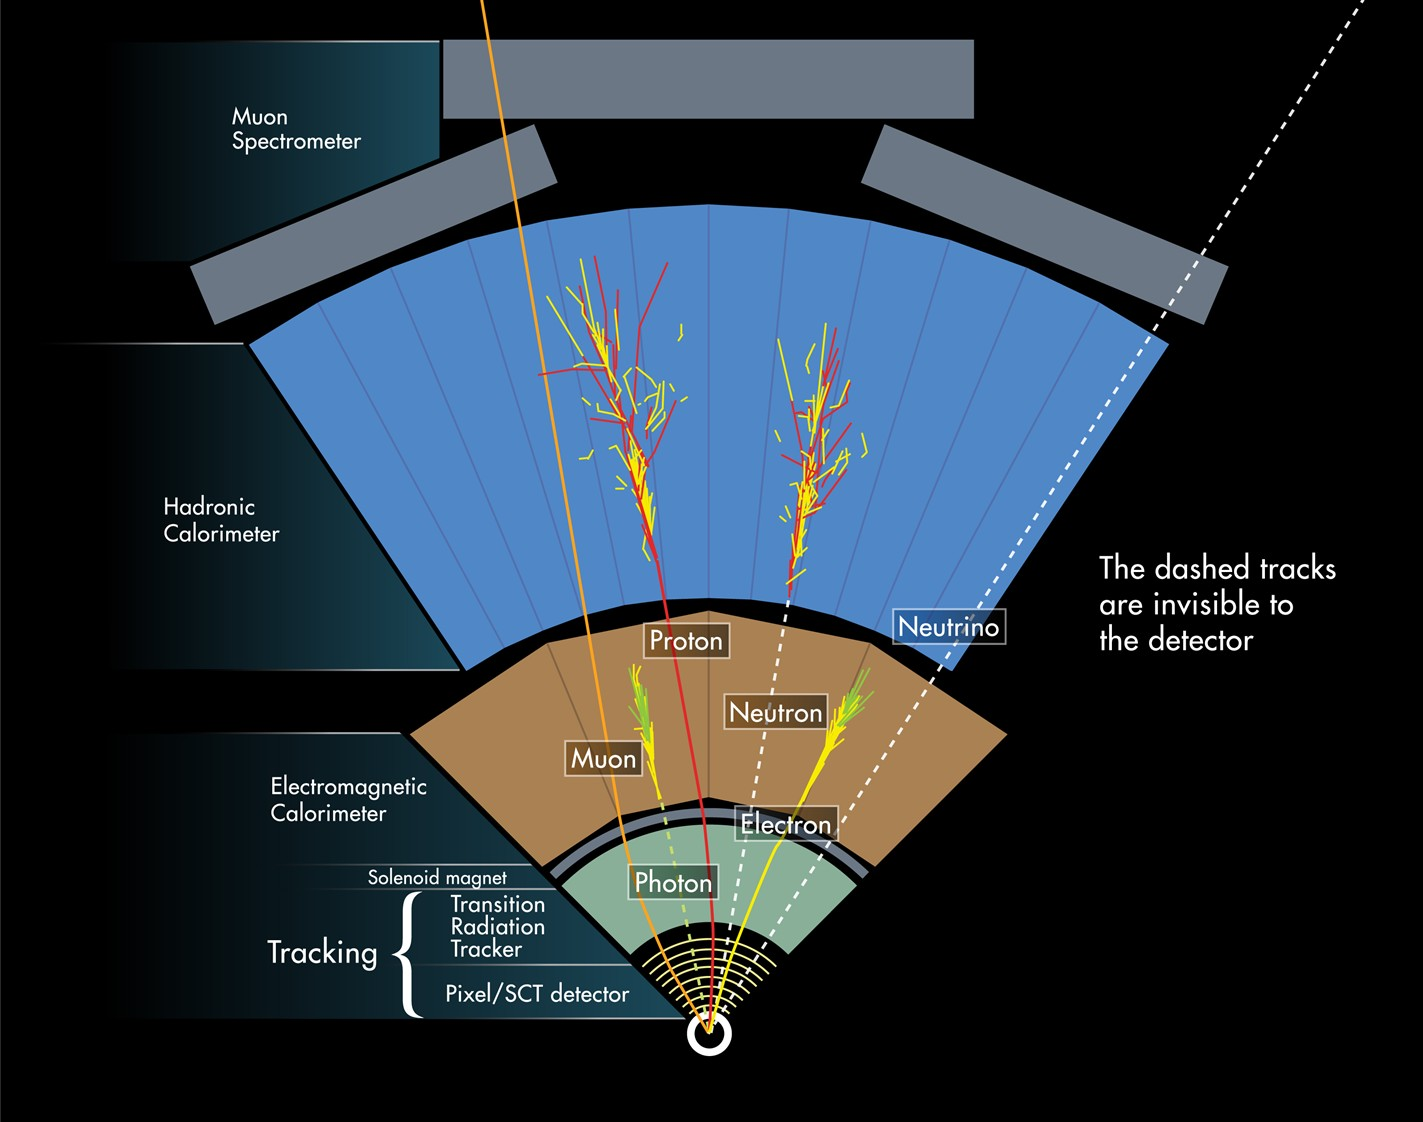
\includegraphics[width=0.90\textwidth]{fig/atlas/atlas-wedge.jpg}
  \caption{A computer-generated image representing how the ATLAS detector functions. The transverse paths of different types of particles are shown interacting with different elements of the detector\cite{atlas-wedge}.}
  \label{fig:atlas-wedge}
\end{figure}
\begin{figure}[tp]
  \centering
  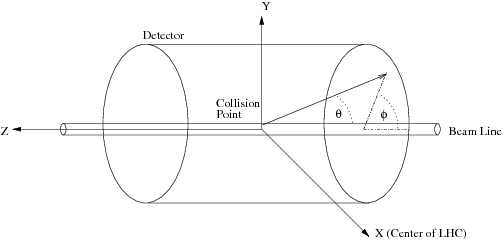
\includegraphics[width=0.90\textwidth]{fig/atlas/coord}
  \caption{Illustration of the ATLAS coordinate system\cite{Schott:2014sea}.}
  \label{fig:atlas-coord}
\end{figure}

\section{Inner detector}
The ID is a series of detectors that functions as a tracking system to measure the momenta and trajectory of charged particles. This also allows reconstruction of the primary and secondary vertices of the collision. The innermost part of the entire detector is the pixel detector, 3 layers of silicon that accurately measure the three-dimensional spatial position of charged particles. Next is the SemiConductor Tracker (SCT), 4 layers of double-sided silicon strip modules which accurately measure tracks in the $r-\phi$ plane and are double sided to provide stereo information along the $z$ axis. The outermost component of the ID is the Transition Radiation Tracker (TRT), straw tubes filled with Xenon gas interleaved with polymer layers which provides additional trajectory measurement and differentiate between electron and hadrons. Figure~\ref{fig:atlas-id} shows a schematic illustration of the ID.

\begin{figure}[tp]
  \centering
  \includegraphics[width=0.7\textwidth]{fig/atlas/id-schem}
  \caption{Schematic view of the Inner Detector: an $r-z$ slice of the cylindrival barrel, disc endcaps with support tubes, and the solenoid magnet. Lines of constant $\eta$ are drawn~\cite{cern-jinst-atlas}.}
  \label{fig:id-scheme}
\end{figure}
\begin{figure}[tp]
  \centering
  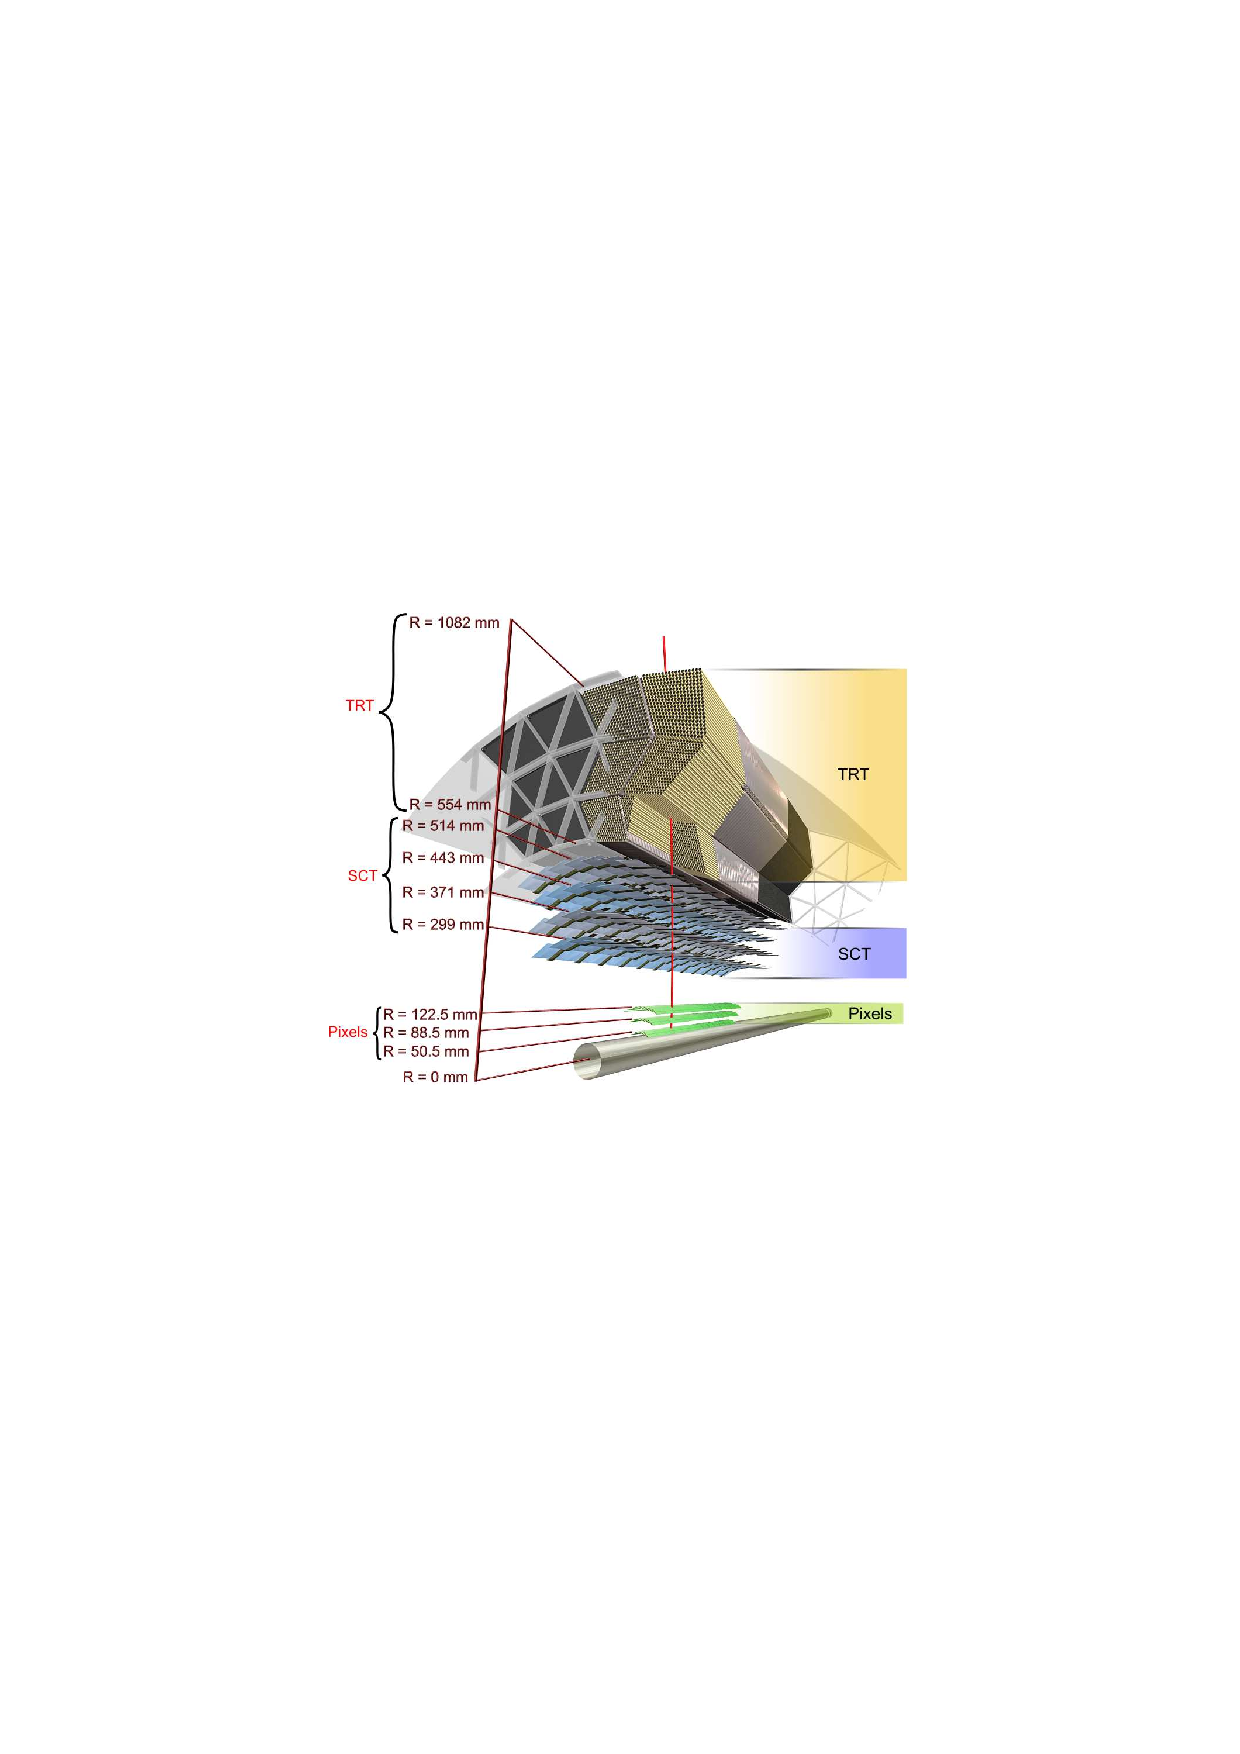
\includegraphics[width=0.7\textwidth]{fig/atlas/id-barrel}
  \caption{A diagram of the barrel of the Inner Detector: the three layers in the Pixels, the four layers in the SCT, and the many layers of the TRT~\cite{cern-jinst-atlas}.}
  \label{fig:id-barrel}
\end{figure}
\subsection{Pixel detector}
\subsection{SemiConductor Tracker}
\subsection{Transition Radiation Tracker}
\subsection{Track reconstruction}
\section{Calorimeters}
\subsection{Electromagnetic calorimeter}
\subsection{Hadronic calorimeter}
\section{Muon spectrometer}
\section{The trigger system}
\subsection{Electron trigger}
\subsection{Muon trigger}